\documentclass[lettersize,journal]{IEEEtran}
\usepackage{amsmath,amsfonts}
\usepackage{algorithmic}
\usepackage{algorithm}
\usepackage{array}
\usepackage[caption=false,font=normalsize,labelfont=sf,textfont=sf]{subfig}
\usepackage{color}
\usepackage{textcomp}
\usepackage{stfloats}
\usepackage{url}
%\usepackage[justification=centering]{caption}
\usepackage{caption2}
\usepackage{verbatim}
\usepackage{graphicx}
\usepackage{cite}
% updated with editorial comments 8/9/2021
\makeatletter
\let\NAT@parse\undefined
\makeatother
\usepackage{hyperref}  %hyperref still needs to be put at the end!

\hyphenation{op-tical net-works semi-conduc-tor IEEE-Xplore}
\hypersetup{hidelinks} 
\def\BibTeX{{\rm B\kern-.05em{\sc i\kern-.025em b}\kern-.08em
		T\kern-.1667em\lower.7ex\hbox{E}\kern-.125emX}}
\usepackage{balance}
\begin{document}

\title{DDPTransformer: Dual-Domain With Parallel Transformer Network for Sparse View CT Image Reconstruction
	\thanks{Manuscript created April, 2022; this work was supported in part by the National Natural Science Foundation of China under Grants U21A20469 and 61972274, and in part by the Applied Basic Research Project of Shanxi Province, China under Grant 202103021224066. (Corresponding author: Yan Qiang).}
}
\author{Runrui~Li, Qing~Li, Hexi~Wang, Saize~Li, Juanjuan~Zhao, Yan~Qiang, Long~Wang
	\thanks{Runrui Li, Qing Li, Hexi Wang, Saize Li and Yan Qiang are with the College of Information and Computer, Taiyuan University of Technology, Taiyuan 030024, China. (e-mail: \href{mailto:qq770486267@gmail.com}{qq770486267@gmail.com;} \href{mailto:liqing0059@link.tyut.edu.cn}{liqing0059@link.tyut.edu.cn;} \href{mailto:hahawhx0719@163.com}{hahawhx0719@163.com;} \href{mailto:565291897@qq.com}{565291897@qq.com} \href{mailto:qiangyan@tyut.edu.cn}{qiangyan@tyut.edu.cn}).}
		
	\thanks{Long Wang is with Jinzhong College of Information, Jingzhong 030600, China.(e-mail: \href{mailto:Drakin1988@qq.com}{Drakin1988@qq.com}).}
	\thanks{Juanjuan Zhao is with Jinzhong College of Information, Jingzhong 030600, China, and also with the College of Information and Computer, Taiyuan University of Technology, Taiyuan 030024, China.(e-mail: \href{mailto:zhaojuanjuan@tyut.edu.cn}{zhaojuanjuan@tyut.edu.cn}).}
}
\markboth{IEEE TRANSACTIONS ON COMPUTATIONAL IMAGING}
{\MakeLowercase{\textit{(et al.)}:
DDPTransformer: Dual-Domain With Parallel Transformer Network for Sparse View CT Image Reconstruction}}

%\IEEEpubid{0000--0000/00\$00.00~\copyright~2021 IEEE}
% Remember, if you use this you must call \IEEEpubidadjcol in the second column for its text to clear the IEEEpubid mark.

\maketitle
\begin{abstract}
Computed tomography (CT) is increasingly essential for clinical diagnosis nowadays while X-ray ionizing radiation is harmful and may increase the risk of cancers. Researchers have thus proposed to obtain sparsely sinograms by reducing the number of detectors to reduce the radioactive impact on human body. However, the sparse-view sinograms have some problems including blurring and streak artifacts, which may adversely confuse the diagnostic assessment to some extent. In this paper, we propose a Transformer-based module named DDPTransformer Block to capture the long-term dependencies within the images and reconstruct high-quality CT images from sparsely sampled sinograms. More specifically, we replace the traditional convolution operation with the Parallel Transformers, and augment the edge information of patch blocks by different splits. In addition, considering that the images to be processed are two-dimensioned, we propose the Layer-Conv-Layer (LCL) module to replace the multilayer perceptron (MLP) in Transformer for feature extraction. Finally, with DDPTransformer Block as the backbone, we propose a deep learning model with four stages including Interpolation, Sinogram Domain Subnet, Filtered BackProjection (FBP) and Image Domain SubNet. For training the model, we use the dataset from the `` Low Dose CT Image and Projection Data (LDCT-and-Projection data)". Experimental results show that the proposed model outperforms the state-of-the-art algorithms for various sparsely sampled sinograms and its robustness has been further verified through other datasets. The code and model are publicly available at: \url{https://github.com/MikasaLee/DDPTransformer}.
\end{abstract}

\begin{IEEEkeywords}
Deep learning, sparse view CT reconstruction, Transformer, dual domains.
\end{IEEEkeywords}

\section{Introduction}
\IEEEPARstart{C}{omputed} tomography (CT) has been widely used in clinical, industrial and other fields \cite{2018Deep}because of its ability to visualize the inner part of an object without destroying it. However, the ionizing radiation of CT can be harmful to humans\cite{2012Hall,2015A}, which severely limits its application. In clinical diagnosis, sparse view CT is used to reduce radiation dose and scan time. However, the defects of the projection view bring ill-posed inverse problems\cite{1989Incomplete} to the reconstructed image. Many reconstruction algorithms have been proposed to solve these problems, and they are classified into three categories: (a) sinogram domain pre-processing, (b) iterative algorithm, and (c) image domain post-processing.

Sinogram domain pre-processing first upsamples and denoises sinograms, and then reconstructs them into CT images. Over the past decades, nonlinear smoothing\cite{2004Nonlinear}, structure adaptive filtering\cite{2012Ray} and dictionary learning based image repair\cite{2014Dictionary}have been proposed for upsampling and denoising in the singram domain. Then the classical analytical methods such as filtered back-projection (FBP)\cite{kak2001principles} were used to reconstruct the CT images. However, the performance of these methods often suffer from the sensitivity of the reconstruction to errors from sinogram domain.

Besides the classic back projection and improved FBP, what have been commonly used for image reconstruction are those iterative algorithms in the past several decades. And the quality of CT images has been greatly enhanced especially thanks to the introduction of compressed sensing (CS)\cite{2006Robust, 2006Donoho} into iterative reconstruction. In fact, a great number of iterative algorithms have been proposed for better reconstruction quality including nonlocal means (NLM)\cite{2009Bayesian}, tight wavelet frames\cite{2011Multi}, dictionary learning\cite{2012Low, 2019Convolutional} and low rank\cite{2014Cine}. Among these iterative methods, the most noteworthy is the total variation (TV)\cite{2008Image} and several other versions improved by it\cite{2014Sparse, 2016Statistical, 2013Few}. However, the aforementioned iterative methods require such a high computational cost and sophisticated parameter adjustment that it may be time consuming to compute and difficult to generalize from various scanning schemes or imaging from different human body parts. 

The last category of sparse view CT reconstruction algorithms is image domain post-processing. After the sparse view CT projection data is reconstructed by the analytical methods, the CT image may have problems such as noise and streak artifacts. Thus, some image domain post processing methods are proposed to improve the quality of CT images by making an effort to eliminate these problems. Inspired by sparse representation theory, Aharon et al. applied dictionary learning\cite{2006ksvd} to LDCT denoising, which significantly improved the quality of abdominal images. Considering other information in the spectrum, Han\cite{2016Sparse} et al. proposed a low-rank Hankel matrix (ALOHA) to reconstruct CT images from sparse view. Compared with the previous two categories of methods, the post-processing methods, where the distribution of noise in the image domain cannot be accurately determined, are unable to optimally trade off structure preservation against removing noise. With the improvement of computer hardware performance and the rapid development of deep learning, many successful applications in the field of medical image reconstruction have been promoted. For example, Chen et al. proposed a residual encoder-decoder convolutional neural network (Red-CNN)\cite{redcnn} for LDCT reconstruction. Jin et al. \cite{2016FBPConvNet} proposed a deep convolutional network (FBPconvNet) that combines FBP, U-net and residual learning to remove CT image artifacts while preserving image structure. Eunhee et al. \cite{8332971} combined wavelet transform and deep residual learning to solve low-dose CT noise reduction, and their proposed method won the second place in the 2016 Low-Dose CT Grand Challenge. Wolterink et al. \cite{2017Generative} introduced the generative adversarial network (GAN), in which they made the predicted image obey the same statistical distribution as NDCT by the discriminator network. Yang et al. \cite{2018Low} proposed to recover subtle structures from FBP-reconstructed CT images using a generative adversarial network (WGAN-GP) with Wasserstein distance and perceptual loss. Chen et al. \cite{2018LEARN} developed the steepest gradient descent algorithm and proposed a Learned Experts' Assessment-based Reconstruction Network (LEARN) for sparse view CT. Although these methods have shown good results, however, long-term dependencies within the image (e.g. non-local correlations of objects in the image) are ignored in CNN, causing partial information loss of the image.

Recent years, in order to solve the problem of limited receptive field of CNN, an attention-based encoder-decoder structure-Transformer\cite{vaswani2017attention} was proposed and achieved great success in many computer vision tasks. Dosovitskiy et al. \cite{dosovitskiy2020vit} proposed Vision Transformer (ViT) for image classification, which was the first time Transformer was used in computer vision and topped SOTA on the famous ImageNet datasets \cite{2009ImageNet}. Liu et al. \cite{liu2021Swin} proposed the Swin Transformer to enhance patch edge information through shift windows, which is the main inspiration of this paper. Chen et al. proposed IPT\cite {chen2021pre}, which is the first application of transformer to low-level computer vision tasks. Wang et al. proposed a Transformer model based on U-net architecture \cite{wang2021uformer} for image reconstruction. Luthra et al. \cite{2021Eformer} proposed an edge-enhanced transformer-based model for medical image denoising. Although the above Transformer models perform outstandingly on other computer vision tasks, Transformer has not yet been utilized in the dual-domain CT reconstruction from sparse-view sinogram.

In this paper, we propose a novel model, called DDPTransformer for solving sparse-view dual-domain CT reconstruction. Benefited from global information obtained by Transformer, the proposed method surpasses the state-of-the-art methods and is proved to be effective for dual-domain CT reconstruction. DDPTransformer consists of 4 steps. First we simulate the sinogram from normal sampling by interpolation. Next we optimize the sinogram for simulating normal sampling through the Sinogram Domain SubNet. Then the sinogram is reconstructed into a CT image by FBP, which is still full of streak artifacts and noise, though. Finally, we remove noise and artifacts through Image Domain SubNet to obtain high-quality CT images. Our contributions are summarized as follows:
\begin{itemize}
	\item{We propose a new model based on joint learning of sinogram domain and image domain for solving sparse-view CT reconstruction. The model shows excellent performance on different views and organs, which indicates the robustness of our model.}
	\item{We design a new Transformer-based backbone module: DDPTransformer Block. It effectively solves the problem of limited receptive field based on convolution, and we further extract the edge information of Patch by parallel Transformer.}
	\item{Different from the basic Transformer model (such as ViT) in CV, we design the Layer-Conv-Layer (LCL) module to replace the MLP, which solves the problem of losing some information due to dimensionality reduction. And through experiments we demonstrate the effectiveness of the LCL module.}
\end{itemize}

The rest of the paper is organized as follows. In Section II, we elaborate on the implementation details of DDPTransformer. Plenty of experiments are demonstrated in Section III. In Section IV, we further discuss the robustness of the model. Finally, the remarks on conclusions and future works are presented in Section V.


\section{METHOD}
In this section, we introduce the implementation of the DDPTransformer in detail from its overall architecture to its building process and illustrate the selection of loss functions for its subnet.

\subsection{Overall Network Architecture}

The reconstruction of the CT image from the sinogram can be expressed as the following linear inverse problem
\begin{equation}
\label{eq1}
g = Af+\eta
\end{equation}
where $g$ is the singram (projection data) that has been measured, $f$ is the corresponding high-quality CT image, $A$ is the matrix for modeling the imaging system and $\eta$ is noise. In fact, in 2D CT reconstruction tasks, $A$ is equivalent to the Radon transform of the parallel beam imaging geometry, and it is irreversible. $\eta$ is most probably Poisson noise. Thus, this inverse problem is highly ill-posed. Our goal is to fit this inverse problem\eqref{eq1} with a neural network. We thus design a network architecture, which consists of four stages, as shown in Figure \ref{fig1}(a). First, to simulate the sinogram obtained under normal sampling, we enlarge the number of detectors by using bilinear interpolation on the input sinogram. The sinogram obtained in this way is excessively smooth and introduces more noise. The next step includes a process of multiple iterations through the DDPTransformer Block for denoising and de-smoothing in Sinogram Domain SubNet. Moreover, the global information we obtain through our transformer can offset the missing local features, helping reconstruct the normal sampling sinograms better. The third step is to convert a sinogram to a CT image, yet containing streek artifacts and noise, through Filtered Back Projection (FBP) in the spatial domain. Finally, in the Image Domain SubNet, multiple DDPTransformer Blocks are also used for iteration. Through the convolution operation in the LCL module, artifacts and noise can be effectively resolved, and high-quality CT images can be finally obtained. Among the four stages of DDPTransformer, the Sinogram Domain SubNet in stage 2 and the Image Domain SubNet in stage 4 are two deep neural networks, so we have to train them separately. Figure \ref{fig1}(b) and \ref{fig1}(c) represent the overall architecture of the two sub-networks during training.

\begin{figure}[!t]
	\centering
	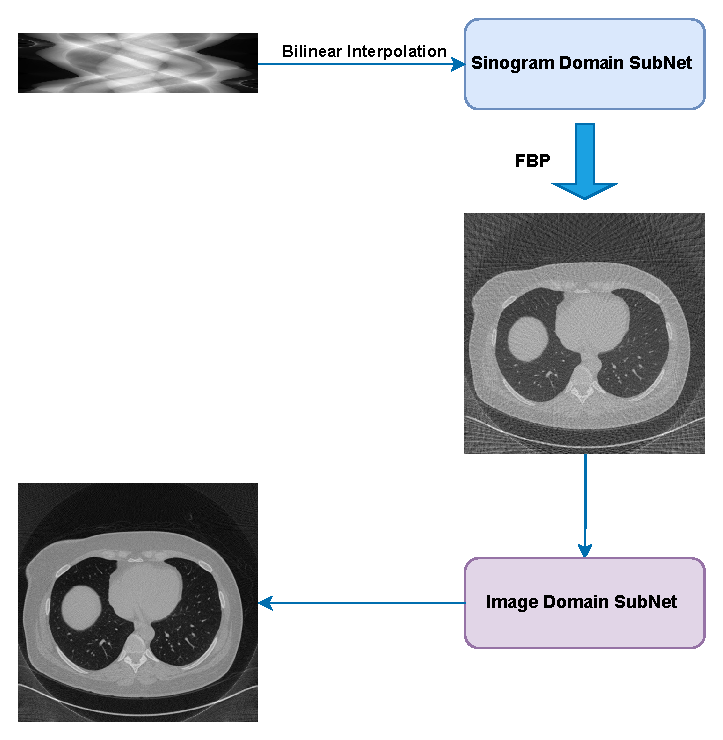
\includegraphics[width=3.5in]{1.eps}
	\caption{The Overall structures of the DDPTransformer, Sinogram Domain SubNet and Image Domain SubNet.}
	\label{fig1}
\end{figure}

In DDPTransformer, both Sinogram Domain SubNet and Image Domain SubNet consist of multiple DDPTransformer Blocks. The overall structure and internal details of the DDPTransformer Block are as follows.

\subsection{DDPTransformer Block Design}

Those past feature extraction based on convolutional neural networks has been proven effective. However, the convolution operation requires continuous accumulation of convolutional layers to complete the extraction of image from local to global information, which can result in shallow convolutional layers not getting too much global information. Instead, the transformer has access to global information from the beginning instead of starting with local information. Although its training becomes more difficult in terms of the size of required dataset and the amount of parameters to be learned, earlier acquisition of global information, as an advantage, may lead to a better result. Our proposed DDPTransformer Block is shown in Figure \ref{fig2}.

\begin{figure*}[!t]
	\centering
	\includegraphics[width=7in]{2.eps}
	\caption{Detailed architecture of DDPTransformer Block.}
	\label{fig2}
\end{figure*}

First we divide the input image $x \in \mathbb{R}^{H\times W \times C}$ into blocks of the same size (e.g. in Figure \ref{fig2} we divided 16 Patches), and operate according to two different division schemes, where $(H, W)$ is the size of the input image x, and $C$ is the channel. One division scheme sets $shift=0$ (as marked in the yellow rectangular box in Figure \ref{fig2}) and divides the input image $x$ into 16 grids, each denoted by $x_p \in \mathbb{R}^{\frac{H}{4}\times \frac{W}{4} \times 16C}$. Then, because the input received by the standard Transformer is a one-dimensional sequence, we flatten each $x_p$ to $x_d \in \mathbb{R}^{N \times 16C}$, where$N = \frac{H\times W}{16}$ is the length of each $x_d$. And with reference to Vision Transformer, we add position embeddings to each sequence to preserve the relative position information. The other division scheme sets $shift=\frac{patch\_size}{2}$ (as marked in the purple rectangular box), and first shift the image $x$ toward right and bottom by $\frac{patch\_size}{2}$, respectively, to get $x'$, as shown in the shaded part of Figure \ref{fig2}. After that, we see that $x$ and $x'$ have overlapping patches. Then we fix the overlapping part and extend the grid lines of $x'$ and border lines of $x$ to divide the rest part in $x$ such that $x$ and $x'$ have matched patches of the same size outside the overlapping part. Next we shift  the corresponding grids from $x$ to $x'$. For example, we shift $A1$ from $x$ to $x'$, $B1$ from $x$ to $x'$, and so forth. After finishing all the shifts, we obtain 16 even patches $x_p \in \mathbb{R}^{\frac{H}{4}\times \frac{W}{4} \times 16C}$ and, as we do in the first scheme, flatten $x_p$ to $x_d \in  \mathbb{R}^{N \times 16C}$ and add position embeddings.

We input the one-dimensional sequences obtained by the two schemes into the Transformer respectively. As shown in Figure \ref{fig3}(a), the Transformer consists of a standard multi-head self attention (MSA) module and a Layer-Conv-Layer (LCL) module (as shown in Figure \ref{fig3}(b)). A layer normalization (LN)\cite{ba2016layer} is used before each module, and a Skip Connection is used after each module.

\begin{figure}[!t]
	\centering
	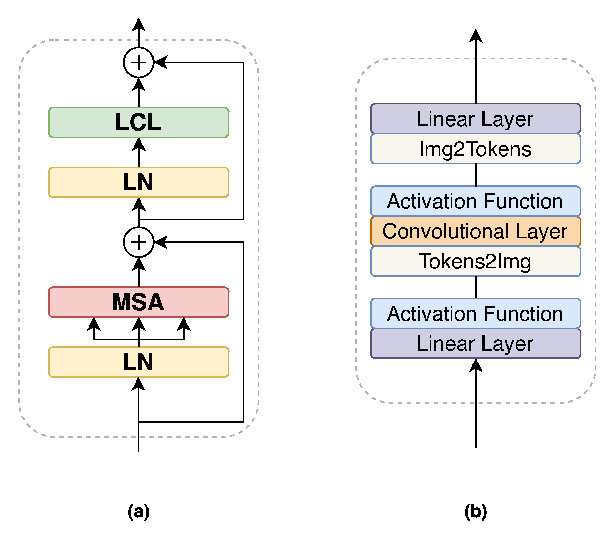
\includegraphics[width=2.5in]{3.eps}
	\caption{Transformer and LCL structure.}
	\label{fig3}
\end{figure}
So the Transformer calculation can be formulated as:
\begin{equation}
\begin{aligned}
\label{eq2}
&x_{d-1} = \{x^1_{d-1}, x^2_{d-1}, \cdots, x^n_{d-1}\},  \mathrm{n\;=\;number\;of\;patches}\\
&y^i_{d-1} = Attention(x^i_{d-1}w^q, x^i_{d-1}w^k, x^i_{d-1}w^v), \mathrm{i=1, 2, \cdots, n} \\
&\hat{x}_{d} = \{y^1_{d-1}, y^2_{d-1}, \cdots, y^n_{d-1}\}, \mathrm{n\;=\;number\;of\;patches}
\end{aligned}
\end{equation}
where $w^q$, $w^k$, $w^v$ represent the projection matrices of query, key and value, respectively. Attention formula is:
\begin{equation}
\label{eq3}
\begin{aligned}
Attention(Q, K, V) = SoftMax(\frac{QK^T}{\sqrt{D}})V
\end{aligned}\end{equation}
where D represents the dimension of query. The formula \eqref{eq2} is to calculate the self-attention of one head, if the number of heads is $k$, then the formula \eqref{eq2} is repeated $k$ times to get $\{\hat{x}^1_{d},\hat{x}^2_{d},\cdots,\hat{x}^k_{d}\}$, and concatenate them to get the final MSA output $\hat{x}_{d}$. And to keep the calculation and the number of parameters constant, D needs to be divided by k.

\textbf{Layer-Conv-Layer (LCL)}. The MSA module focuses on integrating more global information but is incapable of how to learn this information. Hence, we make up for the learning ability through the LCL module. Since the output of MSA is a 1-D sequence, most Transformers are learned by MLP. Although we add relative position information to offset some feature loss caused by dimensional reduction from 2-D to 1-D, the better solution, we think, is to learn directly on 2-D. So we get the LCL module by adding convolution to the MLP. As LCL module architecture is shown in Figure \ref{fig3}(b), we first use Linear Layer and activation function for $\hat{x}_d$, then reshape it to 2-D and use convolution and activation function for learning, and finally flatten back to 1-D get the output by using Linear Layer again.

We concatenate the two schemes ($shift=0$ and $shift=\frac{patch\_size}{2}$) after they were processed by Transformer respectively. The two schemes are used to complement each other's edge information of the patches, so we choose to reshape it into 2-D instead of directly complementing it on 1-D. Finally, the output is obtained by Point-Wise Convolution\cite{2017Xception}.

\subsection{Sinogram Domain SubNet}
\begin{figure*}[!t]
	\centering
	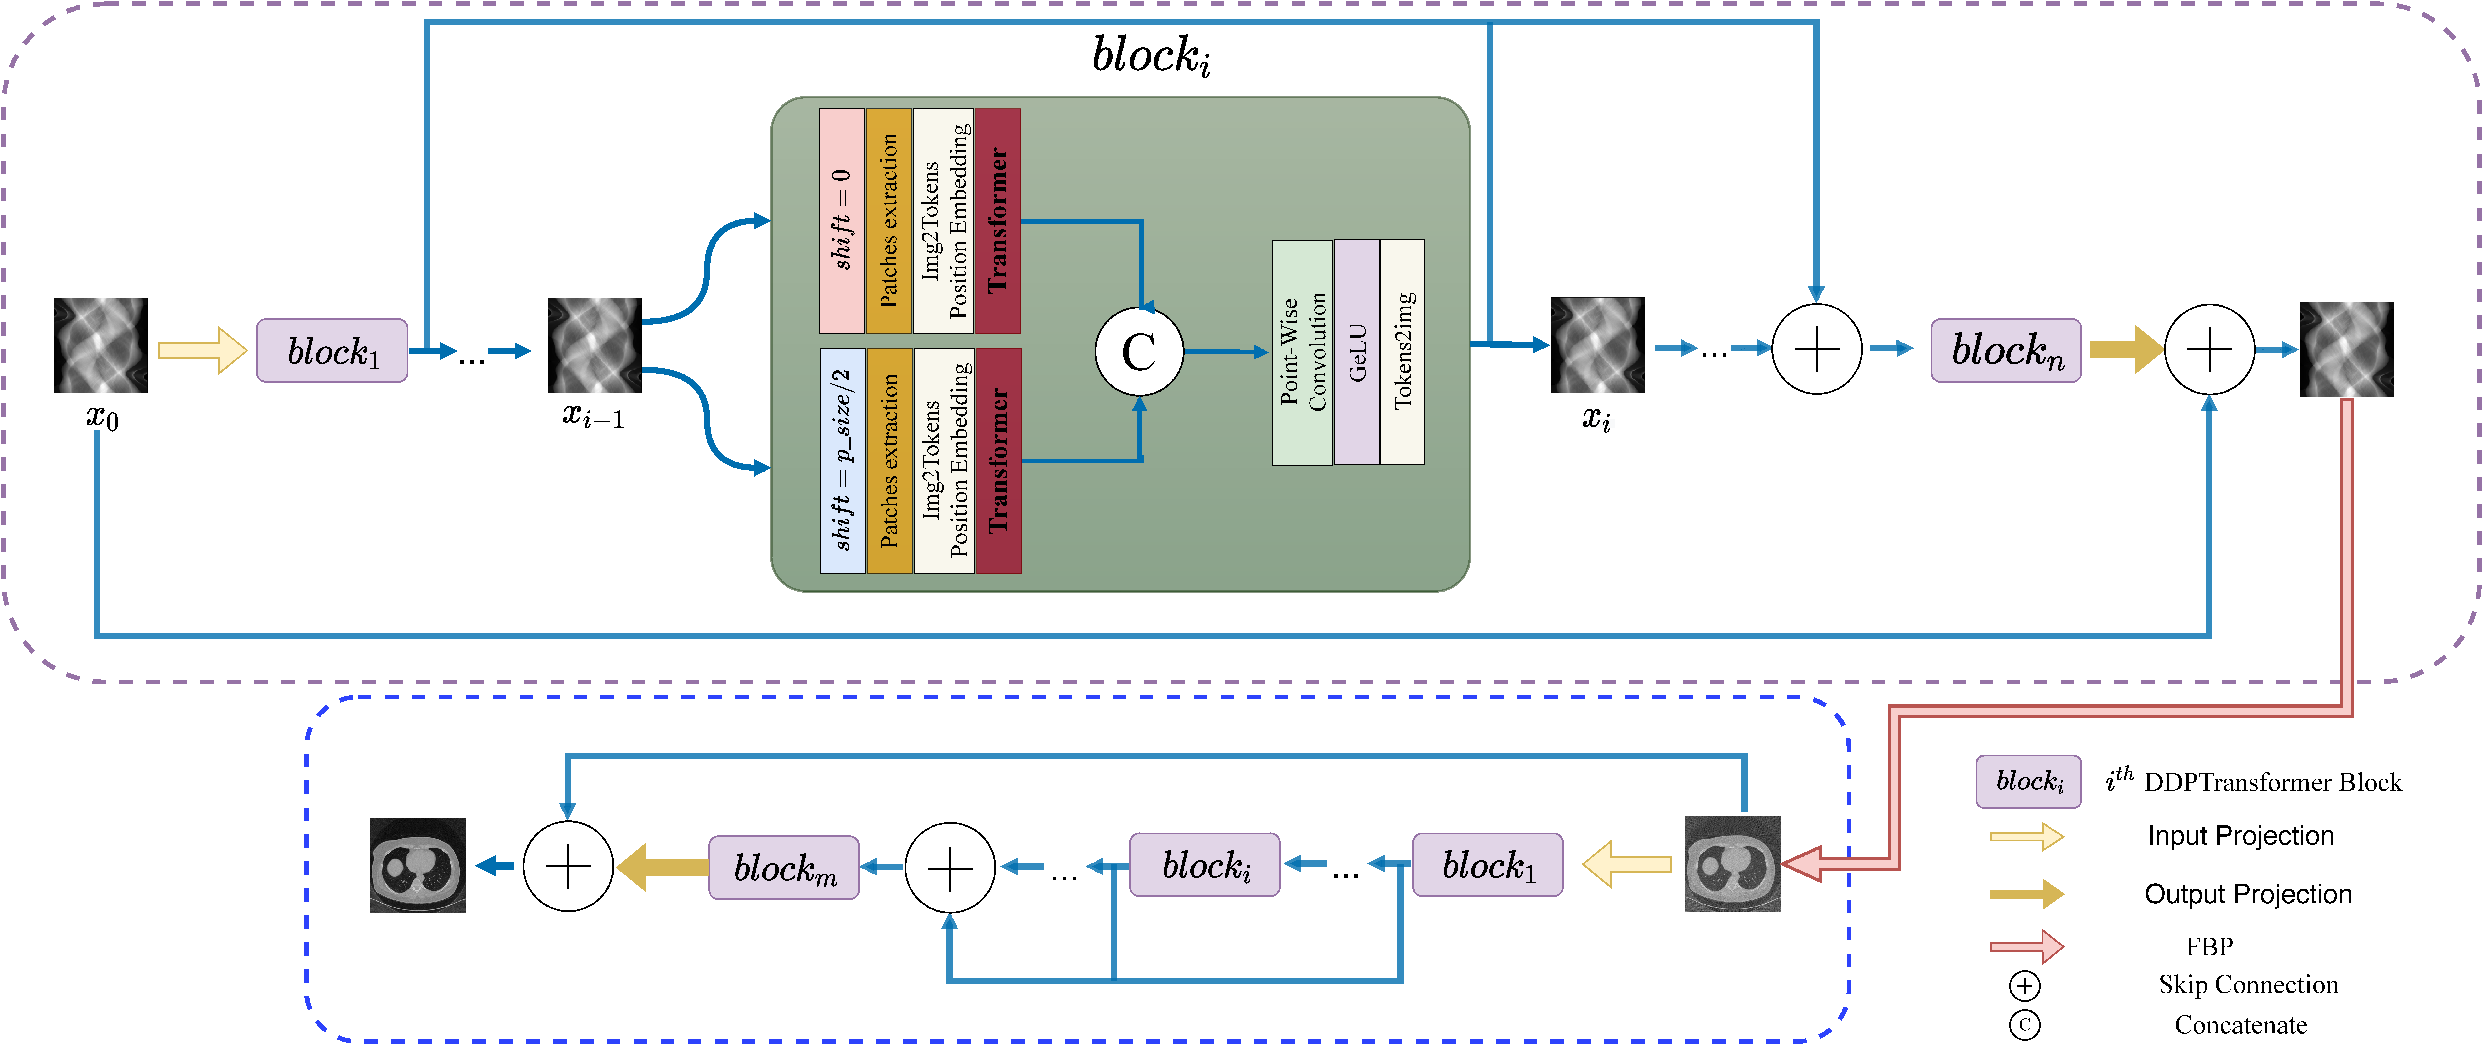
\includegraphics[width=7in]{4.eps}
	\caption{Architecture of the proposed DDPTransformer. The purple dotted box is the Sinogram Domain SubNet. The blue dotted box is the Image Domain SubNet.}
	\label{fig4}
\end{figure*}

As shown in the purple dotted box in Figure \ref{fig4}, Sinogram Domain SubNet uses a flow-based architecture, which consists of 3 parts. First, the interpolated sinogram image is expanded by Input Projection and each channel is flattened into the 1-D token. Next we use $n$ DDPTransformer Blocks as the backbone of Sinogram Domain SubNet, we choose the best value of $n$ through experiments. And using skip connections makes the model easier to fit. Finally, output the 1-D token through Output Projection to get the sinogram under normal sampling. In training Sinogram Domain SubNet, we use the mean square error (MSE) as our loss function:
\begin{equation}
MSE_{Loss}(X^{'},Y) = \mid X^{'}-Y\mid^{2}
\end{equation}
where $X^{'}$ represents the CT image calculated by the model and obtained through the FBP algorithm, and $Y$ is the corresponding high-quality CT image (label).

\subsection{Image Domain SubNet}

Since the CT images reconstructed by FBP are degraded by streak artifacts and noise, we use Image Domain SubNet to reconstruct high-quality CT images. As shown in the blue dotted box in Figure \ref{fig4}, the overall architecture of Image Domain SubNet is similar to Sinogram Domain SubNet. The difference is that we use $m$ DDPTransformer Block modules, and the optimized $m$ will be obtained through experiments. To speed up the convergence of the model as well as to make the model performance better, we use Charbonnier Loss\cite{2017Fast} as the loss function:
\begin{equation}
Charbonnier_{Loss}(X^{'}, Y) = \sqrt{(X^{'}-Y)^{2} + \epsilon^{2}}
\end{equation}
where $X^{'}$ represents the CT image we finally reconstructed and $Y$ is the corresponding high-quality CT image (label). The value of $\epsilon$ is the constant $10^{-3}$.


\section{Experiments}
\subsection{Datasets and Experimental Environment}

We used the ``\emph{Low Dose CT Image and Projection Data (LDCT-and-Projection-data)}"\cite{moen2021low} public dataset provided by the Mayo Clinic in 2020. It contains 25,908 high-quality CT images of 1 mm thickness from 150 cases. The scanning geometry is a fan beam X-ray source with 512 projected views equally distributed around 360$^{\circ}$ and 512 detector elements. The full dose Mayo data were scanned under the protocol 120 kVp and 225 effective mAs (500mA/0.45s). The reference image was generated from 512 projected views using the FBP method, and we simply downsampled the projected data to 128 and 64 views to simulate the sparse view case with a sampling rate of 1/4 and 1/8 respectively. The 150 cases were 50 head cases (labeled N for neuro), 50 chest cases (labeled C for chest) and 50 abdominal cases (labeled L for liver). We randomly selected 40 head cases, 40 chest cases and 40 abdominal cases as the training set and 5 head cases, 5 chest cases and 5 abdominal cases as the validation set, and then used the remaining 5 head cases, 5 chest cases and 5 abdominal cases as test set. Finally, the total number of training set under each view is 20800, the total number of validation set is 2586, and the total number of test set is 2522.

\textbf{Implementation details}: We select a convolution layer with a kernel size of ${4}\times{4}$ and a channel number of 32, and set stride to 4 for saving storage. In Output Projection, we select a transposed convolution layer with the same settings as the convolution layer. After the convolution of Input Projection and Output Projection, we use LeakyReLU\cite{2013Rectifier} to stabilize our training. For each DDPTransformer Block, we choose the MSA with 16 heads, and set the size of the hidden layer four times the input in LCL for better learning. We use Dropout\cite{2014Dropout} with parameter 0.2 to prevent overfitting. Finally, we initialize the weights in the convolutional layers with the Normal Distribution ($\mu$= 0.0, $\sigma$= 0.02). DDPTransformer is trained by Adam algorithm\cite{2014Adam}$\beta_1=0.9$,$\beta_2=0.99$, the learning rate slowly decreases from the initial value $3\times10^{-4}$ to $1\times10^{-6}$. The model was trained for up to 50 epochs and the mini batch size was set to 4. All the experiments were conducted under the environment of Python 3.8 + PyTorch 1.7.1 on a PC (Ubuntu 20.04 + Intel Xeon Silver 4210R CPU + 64G RAM + two NVIDIA RTX A5000 GPUs). The training time might be long due to the huge amount of parameters and the computational complexity and we thus used DistributedDataParallel (DDP) provided by PyTorch to shorten the training time as much as possible. In addition, we implement the FBP algorithm on PyTorch through torchRadon\cite{torch_radon}.

\textbf{Quantitative evaluation metrics}: To verify the effectiveness of our method, the results of network training need to be evaluated. In the field of image reconstruction, there are both subjective and objective evaluation of the quality of images. Commonly used objective evaluation methods are: Peak Signal-to-Noise Ratio (PSNR), Structural Similarity (SSIM) and Root Mean Squared Error (RMSE).

RMSE can compare the prediction errors of different models under a specific data set according to the degree of dispersion of the samples. The smaller the RMSE value, it means the smaller the prediction error of the model. And considering that the value of RMSE is too small, we magnify it 100 times for display, the final definition is as follows:
\begin{equation}
\mathrm{RMSE(X, Y)*100} = 100\times \sqrt{\frac{1}{N}\sum_{i}^N (X_i - Y_i)^2}  
\end{equation}
where $X$ represents the reconstruction result, $Y$ represents the corresponding reference image, and $N$ is the number of pixels in a single image. PSNR is measured on the entire image, and its value is closely related to all pixel values in the image location space whose quality is measured according to the error between the corresponding pixels. The larger PSNR value indicates the larger proportion of useful information in the image and the higher quality of reconstructed CT image. The PSNR formula is as follows:
\begin{equation}
\mathrm{PSNR}(X, Y) = 20\times\log_{10}(\frac{MAX(X,Y)}{RMSE})
\end{equation}
where $MAX(X, Y)$ represents the maximum value of $X$ and $Y$. SSIM evaluates the image quality by considering brightness, contrast and structure comprehensively. The higher the SSIM value, the smaller the image distortion and the better the visual effect of the reconstructed image. The SSIM formula is as follows:
\begin{equation}
SSIM(X, Y) = \frac{(2\mu_x\mu_y+c_1)(2\sigma_{x, y}+c_2)}{(\mu^2_x+\mu^2_y+c_1)(\sigma^2_x+\sigma^2_y+c_2)}
\end{equation}
where $\mu$ represents the average value of the image, $\sigma^2$ represents the variance of the image and $\sigma_{x, y}$ represents the covariance of the two images. $C_1 = (0.03\times R)^2$ and $C_2 = (0.01\times R)^2$ are two constants used to stabilize division with weak denominators, where $R$ represents the value range of image $X$. The image size used to calculate SSIM is $512\times 512$.

\subsection{Quantitative Comparisons}
\begin{table*}[!t]
	\caption{Performance evaluation results of different methods (means $\pm$ standard deviations), the best PSNR value is marked in red.}\label{tab1}
	\centering
	\begin{tabular}{cccc|ccc}
		\hline
		method & PSNR & SSIM & RMSE*100 & PSNR & SSIM& RMSE*100 \\ 
		\hline
		& \multicolumn{3}{c|}{64 views} & \multicolumn{3}{c}{128 views} \\ \hline
		FBP & 20.3683$\pm$0.3074 
		& 0.3141$\pm$0.0113 
		& 1.2390$\pm$0.0831
		& 24.8409$\pm$0.2854 
		& 0.5076$\pm$0.0115
		& 0.4033$\pm$0.0261 \\
		bilinear+FBP 
		& 21.4815$\pm$0.1842
		& 0.5326$\pm$0.0182
		& 0.7301$\pm$0.0307
		& 25.0491$\pm$0.2243
		& 0.6682$\pm$0.0215 
		& 0.3195$\pm$0.0164 \\
		FBPConvNet 
		& 27.7944$\pm$0.1953 
		& 0.6584$\pm$0.0074 
		& 0.1729$\pm$0.0076
		& 34.1109$\pm$0.3703
		& 0.8635$\pm$0.0104
		& 0.0398$\pm$0.0033 \\
		DD-Net 
		& 26.8456$\pm$0.2214
		& 0.6415$\pm$0.0089 
		& 0.2132$\pm$0.0110
		& 33.0648$\pm$0.3304
		& 0.8320$\pm$0.0102
		& 0.0512$\pm$0.0041 \\			
		DP-ResNet 
		& 23.5609$\pm$0.2156
		& 0.6210$\pm$0.0194
		& 0.4469$\pm$0.0221
		& 29.8236$\pm$0.3308
		& 0.7437$\pm$0.0195
		& 0.1076$\pm$0.0085 \\
		Adaptive-Net 
		& 24.2013$\pm$0.3093 
		& 0.6462$\pm$0.0290
		& 0.3856$\pm$0.0275			
		& 31.7390$\pm$0.6146
		& 0.7853$\pm$0.0271 
		& 0.0692$\pm$0.0095 \\
		EEDeepNet 
		& 23.4033$\pm$0.2300 
		& 0.5975$\pm$0.0247
		& 0.4636$\pm$0.0246 
		& 34.2305$\pm$0.6116 
		& 0.8707$\pm$0.0148 
		& 0.0388$\pm$0.0052 \\
		DDPTransformer 
		& \textcolor{red}{29.6453}$\pm$0.9910
		& \textcolor{red}{0.7590}$\pm$0.0495
		& \textcolor{red}{0.1129}$\pm$0.0236
		& \textcolor{red}{34.8335}$\pm$1.8713
		& \textcolor{red}{0.8731}$\pm$0.0385
		& \textcolor{red}{0.0362}$\pm$0.0126 \\ 
		\hline
	\end{tabular}
\end{table*}

To further validate the reconstruction performance of the proposed method in this paper, quantitative analysis is performed in this subsection by comparing the proposed method
with several other reconstruction algorithms in sparse-view CT
reconstruction, including FBPConvNet\cite{2016FBPConvNet}, DD-Net\cite{2018DDNet}, DPResNet\cite{2019DP-ResNet}, Adaptive-Net\cite{2020ADAPTIVE} and EEDeepNet\cite{2020An}. FBPConvNet is a post-processing method that adopts U-Net\cite{2015Unet} to reduce artifacts in FBP reconstruction. DD-Net combines the advantages of DenseNet and Transposed Convolution, applying shortcut connections to concatenate DenseNet and Transposed Convolution to speed up the training of the network. DP-ResNet is a dual-domain network for CT image reconstruction. The algorithm processes the input measurement data separately in the projection domain and the image domain, and uses FBP to connect the two sub-networks. AdaptiveNet customizes a specific network layer with constant weights, and can directly reconstruct CT images from sinograms by integrating the analytical domain transformation knowledge. Feature extraction is performed simultaneously in the singram domain and CT image domain. EEDeepNet is an end-to-end deep network for CT image reconstruction that directly maps sparse sinograms onto CT images. Since the original paper does not name the proposed network, we abbreviate the title of the paper `` End-to-End Deep Network " as EEDeepNet to represent the network proposed in the paper. All training parameters for the comparison experiments are fully referenced to the settings in the original paper or code. Table \ref{tab1} shows the means and the standard deviations of PSNR, SSIM and RMSE$\times100$ of the CT images reconstructed from the test set for the six models at different sampling (views = 64 and 128), and two reference values (FBP and bilinear+FBP) are also listed without model calculation. To better compare the results, we mark the optimal PSNR value of each metric with red in the table. It can be seen that our network obtains the highest PSNR and SSIM values and the lowest RMSE values for different scan settings, which means that our network can reconstruct higher quality CT images. By comparing with the second highest, the PSNR of our method is higher by 1.85dB (64 views) and 0.7dB (128 views) for different samples. Excluding the two reference values without model optimization, FBPConvNet has achieved very good results in all evaluation metrics on 64 and 128 views. But it is only an image post-processing method without learning sinogram images analytically so that its reconstructed images have lower quality than DDPTransformer. The evaluation metrics of DP-ResNet and AdaptiveNet are very poor because we use a much larger sample of dataset than other common datasets, resulting in insufficient network fitting ability for the smaller models. EEDeepNet performs well on 128 views in terms of the evaluation metrics but the worst on 64 views, which indicates that this method has poor robustness to different views.

\subsection{Qualitative Comparisons}

We randomly selected one slice from each of the head, chest and abdomen test dataset and reconstructed them using the selected methods to display the difference among their performance of reconstruction. Figure \ref{fig5} shows the reconstruction results under 64 views, in which the first, second and third rows represent the reconstruction results of the selected head, chest and abdomen slices using different algorithms. To fully compare the reconstruction effect of all selected architectures, we also showed the high quality CT images corresponding to the selected slices of each organ in the figure (original), and marked the region of interest (ROI) with a red rectangle for more detailed analysis. It can be seen that the CT image reconstructed by FBP has serious streak artifacts. Moreover, different models have different degrees of suppression of streak artifacts, and some even reduce image resolution (such as bilinear+FBP and AdaptiveNet). Despite the significant differences between the reconstructed and the original images due to excessively sparse views, DDPTransformer still has the best qualitative results compared to other methods. And by observing the enlarged display of the ROIs in Figure \ref{fig6}, DDPTransformer outperforms other methods profoundly in terms of the reconstruction results for contour and edge information.

\begin{figure*}[!t]
	\centering
	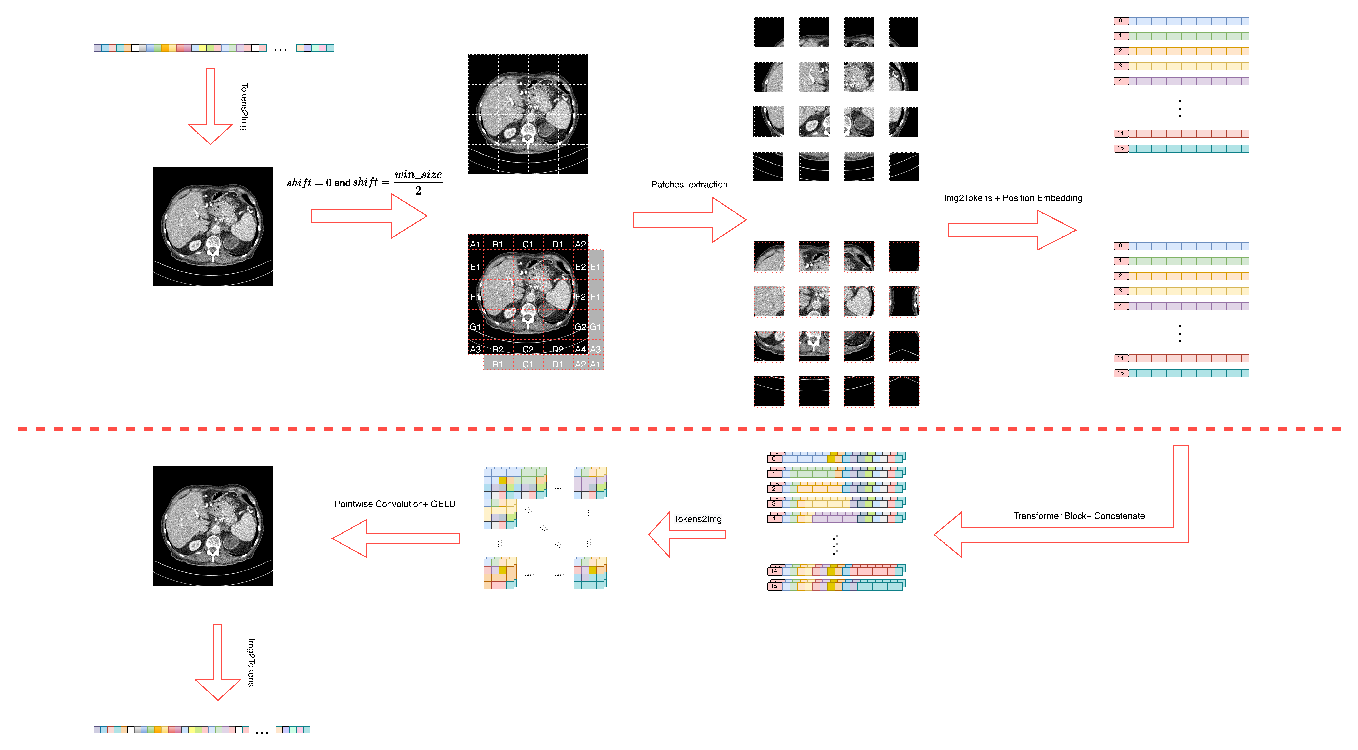
\includegraphics[width=6.5in]{5.eps}
	\caption{CT reconstruction results of different organs under 64 views. where the first row is the head, the second row is the chest, and the third row is the abdomen.}
	\label{fig5}
\end{figure*}
\begin{figure*}[!t]
	\centering
	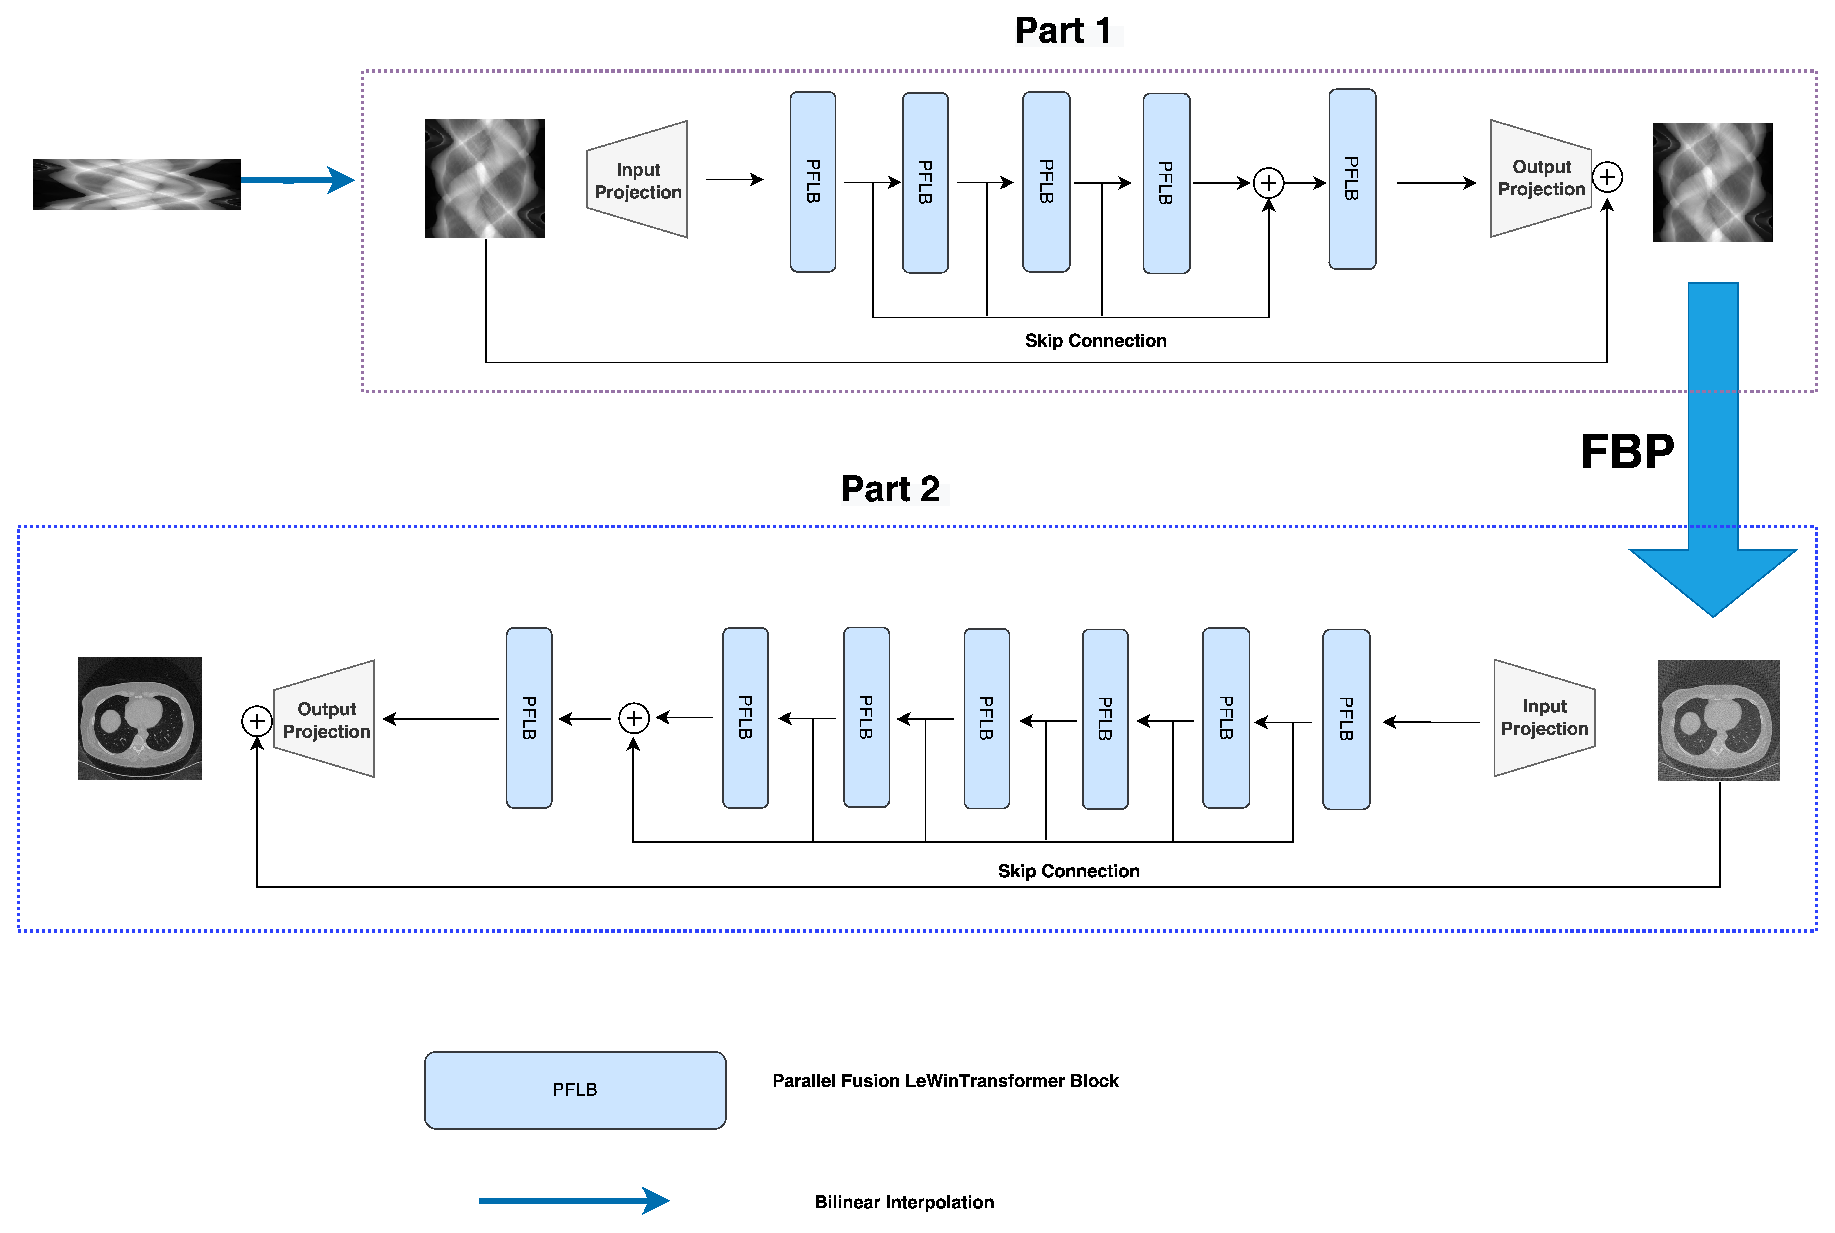
\includegraphics[width=6.5in]{6.eps}
	\caption{Zoom in to show the red rectangle ROI in Figure 5(i)}
	\label{fig6}
\end{figure*}

Figure \ref{fig7} shows the reconstruction results under 128 views. Similarly, the rows 1, 2 and 3 contain the reconstruction results of  the head, chest and abdomen using different algorithms, respectively, and as well show the corresponding high quality CT image with its ROI marked with a red rectangle. It can be seen that the reconstructed images from all models are clearer thanks to the increase of views. Relatively, as we can see, since DPTransformer can get more global information, the results are still the best in terms of clarity and contour of the image and get closer to the original image. According to the enlarged display of the ROIs in Figure \ref{fig8}, although all reconstruction algorithms can reconstruct very clear contours, DDPTransformer can get higher resolution and better visual effects. Finally in Figure \ref{fig9}, we list the quantitative results of all reconstructions in Figure \ref{fig5} and Figure \ref{fig7} for supplementary explanation. The first and second rows represent the different evaluation metrics under 64 and 128 views, respectively, and use red, blue, and green in each histogram to represent the selected head, chest, and abdomen slices.\par
\begin{figure*}[!t]
	\centering
	\includegraphics[width=6.5in]{7.eps}
	\caption{CT reconstruction results of different organs under 128 views, where the first row is the head, the second row is the chest, and the third row is the abdomen.}
	\label{fig7}
\end{figure*}
\begin{figure*}[!t]
	\centering
	\includegraphics[width=6.5in]{8.eps}
	\caption{Zoom in to showed the red rectangle ROI in Figure 7(i)}
	\label{fig8}
\end{figure*}
\begin{figure*}[!t]
	\centering
	\includegraphics[width=6.5in]{9.eps}
	\caption{The quantitative metrics in Figure \ref{fig5} and Figure \ref{fig7}. The first and second rows are the three metrics displayed under 64 and 128 views, respectively, labeled with n for head (neural), c for chest, l for abdomen(liver).}
	\label{fig9}
\end{figure*}

\subsection{Residual Plots}

To further demonstrate the results of the different methods on qualitative analysis, we show the absolute difference image relative to the original image (i.e. residual map) and the residual map of the magnified ROI region, and calculate the relative root mean square error (rRMSE). Its formula is as follows:
\begin{equation}
\mathrm{rRMSE(X,Y)} = \frac{\left\|X-Y\right\|_2}{\left\|Y\right\|_2} \times 100\%   
\end{equation}
where $X$ denotes the reconstructed image and $Y$ denotes the corresponding reference image. The lower rRMSE value represents that the residuals are less weighted in the reference image, which means that the reconstructed image is closer to the reference image. Figure \ref{fig10} shows the residual plots under 64 views, in which the first, second and third rows represent the reconstruction results of the selected head, chest and abdomen slices using different algorithms. The red and blue rectangles represent the magnified ROI and rRMSE value respectively. Since the views are too sparse, the rRMSE of all methods are large and the residual maps obtained from FBPConvNet and DD-Net have significant artifacts. Compared with those of  DP-ResNet, Adaptive-Net and EEDeepNet, the contours of the residual maps obtained by DDPTransformer are much less obvious, indicating a significant improvement in the addition of edge details and the elimination of most artifacts. Furthermore, it turns out that our model has the best qualitative analytical results on 64 views. Figure \ref{fig11} shows the residual plots under 128 views. Similarly, the rows 1 through 3 respectively represent the reconstruction results of the head, chest and abdomen using different algorithms. With more views, the residual plots obtained from each model are better. But the DDPTransformer generates the smallest difference compared to other methods, so that the reconstructed result is closer to the original image. And both 64- and 128-view DDPTransformer achieved the lowest rRMSE value on different human tissues.
\begin{figure*}[!t]
	\centering
	\includegraphics[width=6.5in]{10.eps}
	\caption{Absolute difference images relative to the original image under 64 views.}
	\label{fig10}
\end{figure*}
\begin{figure*}[!t]
	\centering
	\includegraphics[width=6.5in]{11.eps}
	\caption{Absolute difference images relative to the original image under 128 views.}
	\label{fig11}
\end{figure*}

\subsection{Ablation Study}
In the following three subsections, we evaluate the effectiveness of different components in DDPTransformer, such as verifying the effectiveness of Sinogram Domain SubNet (SD-Net) and Image Domain SubNet (ID-Net); finding the best value of the number of DDPTransformer blocks $n$ and $m$ in different subnetworks; and verifying the effectiveness of the Parallel Transformer and LCL modules. By changing one parameter and keeping other parameters unchanged, the optimal value of each parameter is determined. The PSNR, SSIM and RMSE values of all CT images in the test dataset was calculated.

\subsection{Effectiveness of Different SubNets}
\begin{table*}[!t]
	\caption{Quantitative analysis results of each sub-network (means $\pm$ standard deviations).\label{tab2}}
	\centering
	\begin{tabular}{cccc|ccc}
		\hline
		method & PSNR & SSIM & RMSE*100 & PSNR & SSIM& RMSE*100 \\
		\hline  
		& \multicolumn{3}{c|}{64 views} & \multicolumn{3}{c}{128 views} \\
		\hline
		Sinogram Domain SubNet 
		& 28.9623$\pm$0.9575
		& 0.7297$\pm$0.0466
		& 0.1323$\pm$0.0273
		& 33.7763$\pm$1.5785
		& 0.8571$\pm$0.0383
		& 0.0453$\pm$0.0143 \\
		Image Domain SubNet 
		& 29.1686$\pm$0.3456
		& 0.7371$\pm$0.0172
		& 0.1235$\pm$0.0096
		& 33.7571$\pm$0.4986
		& 0.8597$\pm$0.0138
		& 0.0432$\pm$0.0049 \\
		DDPTransformer
		& \textcolor{red}{29.6453}$\pm$0.9910
		& \textcolor{red}{0.7590}$\pm$0.0495
		& \textcolor{red}{0.1129}$\pm$0.0236
		& \textcolor{red}{34.8335}$\pm$1.8713
		& \textcolor{red}{0.8731}$\pm$0.0385
		& \textcolor{red}{0.0362}$\pm$0.0126 \\ 
		\hline
	\end{tabular}
\end{table*}

We tested the performance of SD-Net and ID-Net respectively, and their testing process is shown in Figure \ref{fig1}(b) and Figure \ref{fig1}(c). Table \ref{tab2} lists the means and the standard deviations of the performance evaluation results of SD-Net and ID-Net reconstructed CT images of all test cases under different sampling (views = 64 and 128). It can be seen that the reconstruction result of ID-Net is better than SD-Net. We analyze that there are two main factors that make ID-Net better. For one thing, the CT image itself has more information than sinogram. For another, to learn this information better, the number of DDPTransformer Blocks in ID-Net is more than SD-Net. But it can be seen that no matter which sub-network can not achieve the quantitative results of DDPTransformer.
\subsection{Number of DDPtransformer Blocks}
\begin{figure*}[!t]
	\centering
	\includegraphics[width=6.5in]{12.eps}
	\caption{Line graphs for different values of $n$ and $m$, where the first row shows the test results in SD-Net ($n$) and the second row shows the test results in ID-Net ($m$)}
	\label{fig12}
\end{figure*}

Through experiments, we found the best value of the number of DDPTransformer Blocks $n$ in SD-Net, and the best value of the number of DDPTtransformer Blocks $m$ in ID-Net. Figure \ref{fig12} lists the line graphs of the mean value of all test cases on the quantitative analysis results according to the different values of $n$ and $m$. The test results in SD-Net are denoted in the first row, where we set $n$ from 1 to 7, and it can be seen that all quantitative metrics are getting better when $n$ is in range of 1 to 5 and that the results tend to stable after $n=5$. Hence, we set the optimal value of $n$ as 5. The second row represents the test results in ID-Net. We chose $m$ from 1 to 9 for our experiments, and it turns out that the best results for SSIM on 64 views and for all quantitative metrics on 128 views are acceptable when $m$ is 7, and PSNR and RMSE results on 64 views are also satisfiable. Considering that too many blocks may lead to overfitting of the model, we determined the best value of $m$ as 7.

\subsection{Effectiveness of Different Transformers}

\begin{table*}[!t]
	\caption{Quantitative metrics (means $\pm$ standard deviations) for different Transformers with the best PSNR values marked in red.}
	\label{tab3}
	\centering
		\begin{tabular}{cccc|ccc}
			\hline
			method & PSNR & SSIM & RMSE*100 & PSNR & SSIM& RMSE*100 \\  
			\hline
			& \multicolumn{3}{c|}{64 views} & \multicolumn{3}{c}{128 views} \\ \hline
			Single Transformer+MLP 
			& 27.4160$\pm$0.3170
			& 0.6693$\pm$0.0194 
			& 0.1848$\pm$0.0135
			& 30.9338$\pm$0.4125 
			& 0.7783$\pm$0.0164 
			& 0.0828$\pm$0.0077 \\
			Successive Transformers+MLP
			& 28.4761$\pm$1.0544
			& 0.7039$\pm$0.0537
			& 0.1488$\pm$0.0330 
			& 32.1355$\pm$1.4426
			& 0.8117$\pm$0.0447
			& 0.0656$\pm$0.0188 \\
			Successive Transformer+LCL
			& 27.8340$\pm$0.2849 
			& 0.7104$\pm$0.0170 
			& 0.1677$\pm$0.0107 
			& 32.7085$\pm$0.4841
			& 0.8350$\pm$0.0144
			& 0.0551$\pm$0.0060 \\
			DDPTransformer+MLP
			& 29.1885$\pm$1.0018 
			& 0.7155$\pm$0.0544 
			& 0.1257$\pm$0.0269
			& 32.5042$\pm$1.3632
			& 0.8110$\pm$0.0441
			& 0.0600$\pm$0.0165 \\
			DDPTransformer
			& \textcolor{red}{29.6453}$\pm$0.9910
			& \textcolor{red}{0.7590}$\pm$0.0495
			& \textcolor{red}{0.1129}$\pm$0.0236
			& \textcolor{red}{34.8335}$\pm$1.8713
			& \textcolor{red}{0.8731}$\pm$0.0385
			& \textcolor{red}{0.0362}$\pm$0.0126 \\ 
			\hline
	\end{tabular}
\end{table*}
In this part, we verify the effectiveness of the Parallel Transformer module and LCL module in the DDPTransformer Block respectively. Specifically, the verification operations are: When verifying the impact of the LCL module on the model performance, we change this module to MLP; to verify the impact of Parallel Transformer on model performance, we change it to successive Transformer. In addition, we also listed the single Transformer+MLP and the successive Transformer+MLP as reference values. We made judgments based on the means and the standard deviations of all test set samples on quantitative metrics, and the results are shown in Table \ref{tab3}. After changing the LCL module to MLP, we can see that different quantitative metrics are decreased on different views, which means that LCL can learn more features of the image compared with MLP, and thus can reconstruct better results. After changing the Parallel Transformer to the Successive Transformer, we can see that the quantitative metrics drop more on 64 views. It shows that although the Successive Transformer solves the problem of limited receptive field, the edge information of different Patches is not effectively complementary, resulting in the reconstruction results not as good as DDPTransformer. However, both the LCL module and the parallel Transformer have different degrees of performance improvement compared to the single Transformer+MLP and the successive Transformer+MLP as reference values. The experimental results proved the effectiveness of each module in the DDPTransformer Block.

\section{Discussion}
\begin{table*}[!t]
	\caption{Quantitative metrics results of different methods on the 2016 AAPM dataset (means $\pm$ standard deviations) with the best PSNR values marked in red.}
	\label{tab4}
	\centering
		\begin{tabular}{cccc|ccc}
			\hline
			method & PSNR & SSIM & RMSE*100 & PSNR & SSIM &RMSE*100 \\ 
			\hline
			& \multicolumn{3}{c|}{64 views} & \multicolumn{3}{c}{128 views} \\ 
			\hline
			FBP & 29.9765$\pm$0.1209
			& 0.5416$\pm$0.0063
			& 0.1350$\pm$0.0035
			& 34.4040$\pm$0.0949
			& 0.7454$\pm$0.0061
			& 0.0446$\pm$0.0010 \\
			bilinear+FBP 
			& 30.4448$\pm$0.1365
			& 0.8206$\pm$0.0034
			& 0.0922$\pm$0.0029
			& 34.3314$\pm$0.1436
			& 0.9075$\pm$0.0021 
			& 0.0374$\pm$0.0012 \\
			FBPConvNet
			& 36.9814$\pm$0.1666
			& 0.8939$\pm$0.0032 
			& 0.0206$\pm$0.0008
			& 42.7887$\pm$0.0948
			& 0.9682$\pm$0.0004
			& 0.0054$\pm$0.0001 \\
			DD-Net 
			& 30.4719$\pm$0.0546
			& 0.8525$\pm$0.0015
			& 0.0900$\pm$0.0011
			& 33.7510$\pm$0.0444
			& 0.9039$\pm$0.0010
			& 0.0424$\pm$0.0004 \\			
			DP-ResNet 
			& 31.2974$\pm$0.1674
			& 0.8426$\pm$0.0036
			& 0.0746$\pm$0.0029
			& 35.3386$\pm$0.1026
			& 0.9120$\pm$0.0018
			& 0.0295$\pm$0.0007 \\
			Adaptive-Net 
			& 31.3441$\pm$0.2889
			& 0.8659$\pm$0.0041
			& 0.0738$\pm$0.0050
			& 35.3676$\pm$0.2762
			& 0.9284$\pm$0.0016
			& 0.0293$\pm$0.0018 \\
			EEDeepNet 
			& 32.4082$\pm$0.1377 
			& 0.8714$\pm$0.0024
			& 0.0578$\pm$0.0018
			& 43.9455$\pm$0.1820
			& 0.9750$\pm$0.0006
			& 0.0041$\pm$0.0002 \\
			DDPTransformer 
			& \textcolor{red}{37.0181}$\pm$0.3035
			& \textcolor{red}{0.9270}$\pm$0.0041
			& \textcolor{red}{0.0202}$\pm$0.0014
			& \textcolor{red}{45.1001}$\pm$0.3832
			& \textcolor{red}{0.9787}$\pm$0.0013
			& \textcolor{red}{0.0032}$\pm$0.0003 \\ 
			\hline
	\end{tabular}
\end{table*}
\begin{figure*}[!t]
	\centering
	\includegraphics[width=6.5in]{13.eps}
	\caption{Qualitative metrics on the 2016 AAPM dataset, 64 views in the first row and 128 views in the second row.}
	\label{fig13}
\end{figure*}
\begin{figure*}[!t]
	\centering
	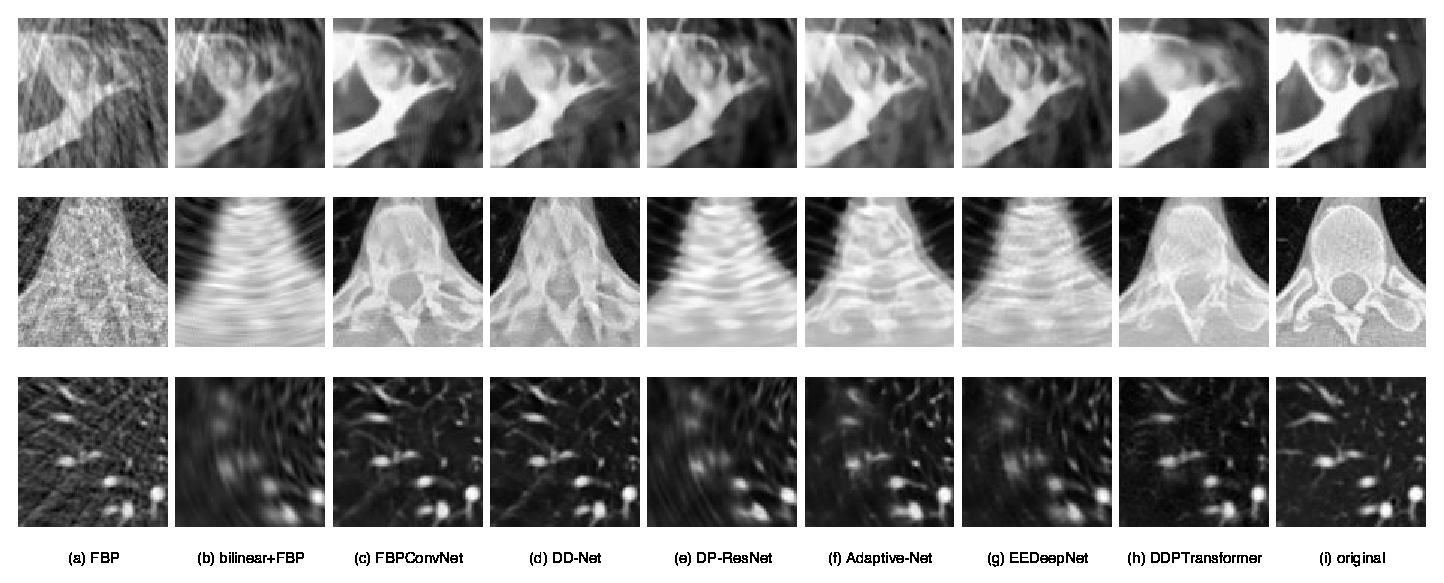
\includegraphics[width=6.5in]{14.eps}
	\caption{Figure \ref{fig13} Quantitative metrics.}
	\label{fig14}
\end{figure*}
\begin{figure*}[!t]
	\centering
	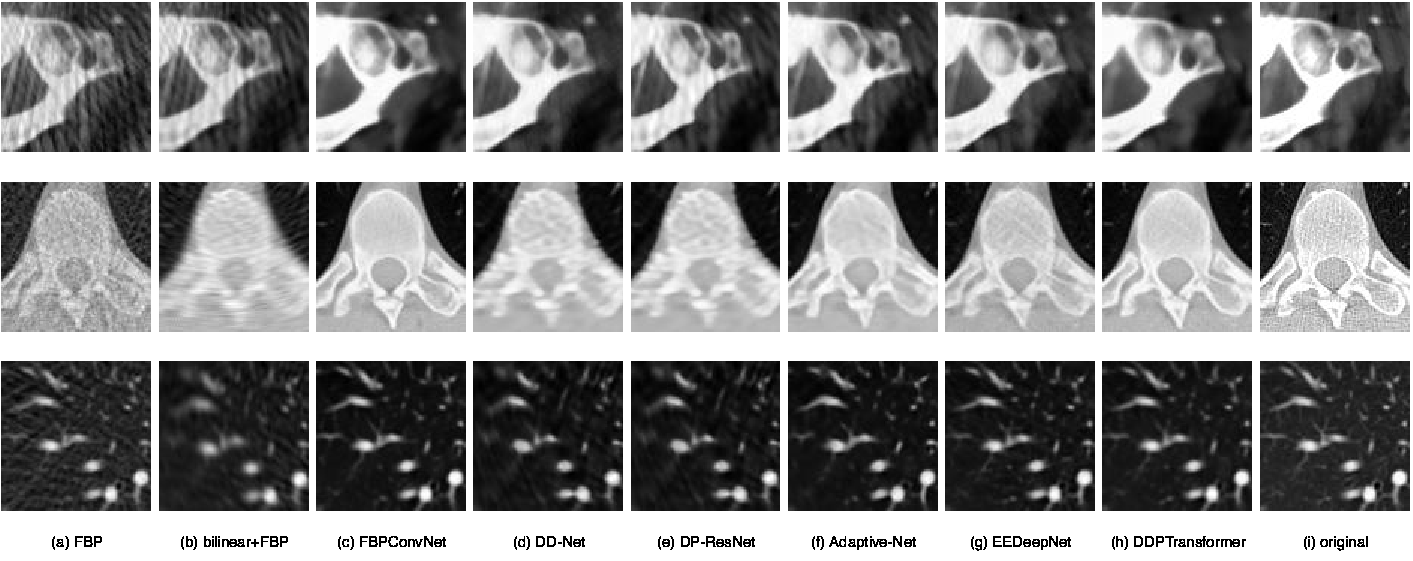
\includegraphics[width=6.5in]{15.eps}
	\caption{Zoom in to show the red rectangle ROIs in Figure \ref{fig11}(i).}
	\label{fig15}
\end{figure*}
\begin{figure*}[!t]
	\centering
	\includegraphics[width=6.5in]{16.eps}
	\caption{Absolute difference images relative to the original image on the 2016 AAPM dataset.}
	\label{fig16}
\end{figure*}
We have demonstrated its excellent performance on ``LDCT-and-Projection-data '' dataset. To further verify the robustness of our model, we randomly selected a total of 1086 slices from two patients from the famous `` \emph{2016 NIH-AAPM-Mayo Clinic Low Dose CT Grand Challenge} " (2016aapm)\cite{mccollough2016tu} dataset for testing. Table \ref{tab4} shows the means and the standard deviations of the quantitative metrics results for all slices tested, and it can be seen that DDPTransformer still works best on the dataset that has not been trained at all. Compared with the second highest, the PSNRs of DDPTransfomer are 0.037dB (64 views) and 1.155dB (128 views) higher respectively under different sparse sampling.  As shown in Figure \ref{fig13}, we randomly selected a slice to display its qualitative metrics. And their quantitative metrics are listed in Figure \ref{fig14}, in which we found through comparison that DDPTransformer is not the best in RMSE value but works the best in terms of PSNR and SSIM and that the overall quality of CT images reconstructed under different views is much higher. By observing the enlarged ROI in Figure \ref{fig15}, it can be seen that the DDPTransformer performs well at handling the details such as edges, contours and streak artifacts and preserving the fine structures. Figure \ref{fig16} shows the absolute difference image relative to the original image and the residual plots of the magnified ROI, and the rRMSEs are calculated. It can be seen that DDPTransformer achieves the best results in both qualitative and rRMSE on different views. In addition, Transformer has a larger number of parameters than CNN, which leads to longer running time. In future research, we will study how to reduce the number of parameters and running time, while further improving the performance of the model with more sparse sampling.

\section{Conclusions}

CT technology has become the most commonly used auxiliary diagnostic method in modern medicine. To avoid the damage caused by CT ionizing radiation, the application under sparse sampling has gained increasing attention. To reconstruct high quality CT images from sparse-view sinograms, we propose a Transformer-based model for sparse-view dual-domain CT reconstruction. We use Transformer to replace convolution to solve the problem of limited receptive field, and solve the problem that the edge information of Patch block is difficult to learn in the parallel way. And replace the MLP by the Layer-Conv-Layer (LCL) module, so that the Transformer can learn more image information over long distances. The experimental results show that the model is suitable for different sparse views and human organs, and achieves the best results in different quantitative metrics such as PSNR, SSIM, and RMSE compared with other reconstruction algorithms. And the model effectively preserve the structure and texture information of CT images while removing noise and artifacts, and obtain satisfactory qualitative metrics. Finally, we further verify its robustness on other datasets, and the results are still the best.

\bibliographystyle{IEEEtran}
\bibliography{ct_reconstruction}
\newpage
\end{document}